\scanpage{283}
\margin{\figure{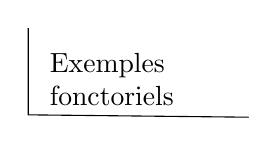
\begin{tikzpicture}\node[align=left,anchor=west] at (0.15,0.45) {\unsure{Exemples}\\fonctoriels};\draw (0,1.1)--(0,0)--(2.8,-0.03);\end{tikzpicture}}}

\diagram{\begin{tikzcd}X\arrow[d,"g"]\\Y\arrow[d,"f"]\\S\end{tikzcd}}

\diagram{\begin{tikzcd}[column sep=small]
&&&\Gamma(\deleted{\unsure{Y,}}\uuline{\operatorname{Pic}}_{X/Y}\unsure{,|/}Y)\arrow[d,equal]\\
0\arrow[r]&\operatorname{Pic}(Y)\arrow[r]&\operatorname{Pic}(X)\arrow[r]&\operatorname{Pic}(X/Y)
\end{tikzcd}}
\deleted{$\unsure{\Gamma(S,\prod_{Y/S}\uline{\operatorname{Pic}})}$}
\margin{surjectif si $X/Y$ a une section}

Pourvu que $g$ soit qu. cpt séparé et $\mathcal O_Y\overset{\sim}{\longrightarrow}g_*(\mathcal O_X)$.

-- Si cette dernière condition est $S$-universelle, alors \deleted{pour} faisant un changement de base quelconque $S'\longrightarrow S$, et passant aux ``faisceaux'' associés dans la suite exacte de \deleted{foncteurs} ``préfaisceaux'' ainsi obtenue, on trouve une suite exacte
\diagram{\begin{tikzcd}
0\arrow[r]&\uuline{\operatorname{Pic}}_{Y/S}\arrow[r]&\uuline{\operatorname{Pic}}_{X/S}\arrow[r]&\prod_{Y/S}\uuline{\operatorname{Pic}}_{X/Y}
\end{tikzcd}},
avec d'ailleurs un zéro à droite \inserted{\unsure{et splitting}} si $X/Y$ a une section. Donc si les foncteurs envisagés sont représentables, on trouve une suite \uline{exacte}
\diagram{\begin{tikzcd}
0\arrow[r]&\uline{\operatorname{Pic}}_{Y/S}\arrow[r]&\uline{\operatorname{Pic}}_{X/S}\arrow[r]&\prod_{Y/S}\uline{\operatorname{Pic}}_{X/Y}
\end{tikzcd}}
où la dernière flèche a un inverse à droite si $X/Y$ a une section. Dans ce cas, ceci donne un isom
\[
\uline{\operatorname{Pic}}_{X/S}\simeq\uline{\operatorname{Pic}}_{Y/S}\times\prod_{Y/S}\uline{\operatorname{Pic}}_{X/Y}
\]
[ceci généralise la relation connue, quand $X=Y\times_S Z$, $Z$ muni d'une section sur $S$
\[
\uline{\operatorname{Pic}}_{X/S}\simeq\uline{\operatorname{Pic}}_{Y/S}\times\uline{\operatorname{Pic}}_{Z/S}\times\uline{\operatorname{Hom}}_{\text{pointé}}(Y,\uline{\operatorname{Pic}}^{\unsure{\tau|0}}_{Z/S})
\]
]
\mspage{282}
